\documentclass[sigconf,natbib=true,anonymous=true]{acmart}
% \documentclass[manuscript,screen,review]{acmart}

% Needed to fix an acmart problem with line numbering. AFAICT line 
% numbers are not expected in sigconf, so it should be a no-op.
\makeatletter
\providecommand{\@LN}[2]{}
\makeatother

% % Fonts used in the template cannot be substituted; margin 
% % adjustments are not allowed.
% %
% % \BibTeX command to typeset BibTeX logo in the docs
% \AtBeginDocument{%
%   \providecommand\BibTeX{{%
%     \normalfont B\kern-0.5em{\scshape i\kern-0.25em b}\kern-0.8em\TeX}}}

%% Rights management information.  This information is sent to you
%% when you complete the rights form.  These commands have SAMPLE
%% values in them; it is your responsibility as an author to replace
%% the commands and values with those provided to you when you
%% complete the rights form.
\setcopyright{acmcopyright}
\copyrightyear{2022}
\acmYear{2022}
\acmDOI{XXXXXXX.XXXXXXX}

%% These commands are for a PROCEEDINGS abstract or paper.
\acmConference[SIGIR '22]{Make sure to enter the correct
  conference title from your rights confirmation email}{June 03--05,
  2018}{Woodstock, NY}
%
%  Uncomment \acmBooktitle if the title of the proceedings is different
%  from ``Proceedings of ...''!
%
\acmBooktitle{SIGIR '22: Proceedings of the 45th International ACM SIGIR Conference on Research and Development in Information Retrieval,
 July 11--15, 2022, Madrid, Spain} 
% \acmPrice{15.00}
% \acmISBN{978-1-4503-XXXX-X/18/06}

%
% Submission ID.
% Use this when submitting an article to a sponsored event. You'll
% receive a unique submission ID from the organizers
% of the event, and this ID should be used as the parameter to this command.
% \acmSubmissionID{123-A56-BU3}

%
% The majority of ACM publications use numbered citations and
% references.  The command \citestyle{authoryear} switches to the
% "author year" style.
%
% If you are preparing content for an event
% sponsored by ACM SIGGRAPH, you must use the "author year" style of
% citations and references.
% Uncommenting
% the next command will enable that style.
%\citestyle{acmauthoryear}

%% The "author" command and its associated commands are used to define
%% the authors and their affiliations.
%% Of note is the shared affiliation of the first two authors, and the
%% "authornote" and "authornotemark" commands
%% used to denote shared contribution to the research.
\author{Ben Trovato}
\authornote{Both authors contributed equally to this research.}
\email{trovato@corporation.com}
\orcid{1234-5678-9012}
\author{G.K.M. Tobin}
\authornotemark[1]
\email{webmaster@marysville-ohio.com}
\affiliation{%
  \institution{Institute for Clarity in Documentation}
  \streetaddress{P.O. Box 1212}
  \city{Dublin}
  \state{Ohio}
  \country{USA}
  \postcode{43017-6221}
}

\author{Lars Th{\o}rv{\"a}ld}
\affiliation{%
  \institution{The Th{\o}rv{\"a}ld Group}
  \streetaddress{1 Th{\o}rv{\"a}ld Circle}
  \city{Hekla}
  \country{Iceland}}
\email{larst@affiliation.org}

\author{Valerie B\'eranger}
\affiliation{%
  \institution{Inria Paris-Rocquencourt}
  \city{Rocquencourt}
  \country{France}
}

\author{Aparna Patel}
\affiliation{%
 \institution{Rajiv Gandhi University}
 \streetaddress{Rono-Hills}
 \city{Doimukh}
 \state{Arunachal Pradesh}
 \country{India}}

\author{Huifen Chan}
\affiliation{%
  \institution{Tsinghua University}
  \streetaddress{30 Shuangqing Rd}
  \city{Haidian Qu}
  \state{Beijing Shi}
  \country{China}}

\author{Charles Palmer}
\affiliation{%
  \institution{Palmer Research Laboratories}
  \streetaddress{8600 Datapoint Drive}
  \city{San Antonio}
  \state{Texas}
  \country{USA}
  \postcode{78229}}
\email{cpalmer@prl.com}

\author{John Smith}
\affiliation{%
  \institution{The Th{\o}rv{\"a}ld Group}
  \streetaddress{1 Th{\o}rv{\"a}ld Circle}
  \city{Hekla}
  \country{Iceland}}
\email{jsmith@affiliation.org}

\author{Julius P. Kumquat}
\affiliation{%
  \institution{The Kumquat Consortium}
  \city{New York}
  \country{USA}}
\email{jpkumquat@consortium.net}

%%%%%%%%%%%%%%%%%%%%
%%%%%%%%%%%%%%%%%%%%
% EDITING LINK: 
% https://www.overleaf.com/3575751412sjsdmszkxsyh
%%%%%%%%%%%%%%%%%%%%
%%%%%%%%%%%%%%%%%%%%

% \usepackage{soul} %% Soul does not play well with acmart
\usepackage{url}
% % \usepackage[hidelinks]{hyperref}https://www.overleaf.com/project/614b5cc61d38655dce466002
% \usepackage[small]{caption}
\usepackage{graphicx}
\usepackage{amsthm}
\usepackage{booktabs}
\usepackage{algorithm}
\usepackage{algorithmic}
\urlstyle{same}

% % =======================================
% % my imported packages

\usepackage{amsmath}
\usepackage{bm}
% \usepackage{amssymb}          % duplicates something in acmart
\usepackage{listings}
% \usepackage[ruled,vlined]{algorithm2e}
\include{pythonlisting}

\newcommand{\pseudosection}[1]{\vspace{1.5ex}\noindent \textit{{#1:~~}}}
% \newcommand{\pseudosection}[1]\indent{{{}}}

\usepackage{todonotes}
\newcommand{\todokdinline}[1]{\todo[color=red!20,inline]{{KD: \small #1}}}
\newcommand{\todokd}[1]{\todo[color=red!20]{{\small #1 -- Kasra}}}
% \newcommand{\todocainline}[1]{\todo[color=yellow!20,inline]{{CA: \small #1}}}
\newcommand{\todocm}[1]{\todo[color=green!40]{\small #1 -- Cynthia}}
\newcommand{\todocmi}[1]{\todo[inline,color=green!40]{\small #1 -- Cynthia}}
\newcommand{\todoff}[1]{\todo[color=blue!20]{\small #1 -- Frank}}
\newcommand{\todoed}[1]{\todo[color=cyan!20]{\small #1 -- Ed}}

\newcommand{\CitationNeeded}[1]{{\textbf {\color{red}Cite #1}}}
\newcommand{\ProofRead}[1]{{\textbf {\color{red}Proofread please #1}}}
\newcommand{\Complete}[0]{{\textbf {\color{red}Complete it }}}
\newcommand{\Rephrase}[1]{{\textbf {\color{red}Rephrase please #1}}}

% \newcommand{\citet}[1]{\cite{#1}} % This is used because \citet didn't work with their author kit % It does now

% =======================================
\title{Multimodal Contrastive Learning for Physical Object Retrieval}

\begin{document}

% Todo list
% \begin{enumerate}
%     \item \st{Lit search}
% \end{enumerate}
% \newpage

% ***************** The BEGINNING of the paper *****************

\begin{abstract}
    % Grounded language understanding, in which natural language is used as a query against objects in a physical environment, allows a real-world, intuitive mechanism by which users can instruct physical agents to engage in tasks such as object retrieval. Visuolinguistic approaches to such object inference tasks typically involve training on large pools of image/text pairs and then using language to subselect elements of the sensed environment. However, physical agents such as robots typically have access to sensory and interactive modalities beyond vision, and learning from multiple modalities can improve performance on downstream tasks. In order to fully leverage multimodal training data while being robust to missing information, we propose a generalized distance-based loss function that can be extended to learn retrieval models that incorporate an arbitrary number of modalities. We demonstrate the usability of our model on a grounded language object retrieval scenario, where an intelligent agent has to select an object given an unconstrained language command. We leverage four modalities including vision, depth sensing, text, and speech, and we show that our model can outperform state-of-the-art contrastive models when modalities are ablated.
    % \todokdinline{Text is easier to learn from compared to speech, and our proposed model allow us to minimize the distance between text and speech and when text is missing during the test time, speech can be used to perform the task, and it outperforms the supervised contrastive learning because such a leverage is missing there.}
    
    % FRANK:
    
    We propose a generalized distance-based loss function that can be used to learn retrieval models that incorporate an arbitrary number of views of 
    a particular piece of data. %
    We study this in the context of grounded language understanding, in which natural language is used as a query against objects in a physical environment, allowing a real-world, intuitive mechanism by which users can instruct physical agents to engage in tasks such as object retrieval.
    In our setting, each view is a different modality of data, such as written text, spoken language, and images. 
    % Visuolinguistic approaches to such object inference tasks typically involve training on large pools of image/text pairs and then using language to subselect elements of the sensed environment. 
    %Such an approach could improve the ability of physical agents, such as robots typically have access to sensory and interactive modalities beyond vision, and learning from multiple modalities can improve performance on downstream tasks.
    We demonstrate the usability of our model on a grounded language object retrieval scenario, where an intelligent agent has to select an object given an unconstrained language command. We leverage four modalities including vision, depth sensing, text, and speech, and we show that our model can outperform state-of-the-art contrastive models when modalities are ablated.
    
\end{abstract}

\settopmatter{printfolios=true} % Page numbers please 
9 pages without references.
%===================================================================

\maketitle
% \setcounter{page}{1}

%===================================================================

% \section{SIGIR Papers}
% \begin{enumerate}
%     \item \href{https://dl.acm.org/doi/pdf/10.1145/3397271.3401430}{FashionBERT}
%     \item \href{https://dl.acm.org/doi/pdf/10.1145/3397271.3401265?casa_token=W8NqNWp0UQkAAAAA:w-iRUnNhmytDKCUiYzaUPG0bI_yyo8Bzxwro_eOC-zl5VDIGRVT2dvixvnCwLJ0iEKqYo1LkQIWXVA}{CrossBERT}
    
% \end{enumerate}

\section{Introduction}
\label{intro}

Humans use multiple sensory inputs to understand, interact with, and retrieve information from the world around them. It is intuitive that agents learning about the world, upon encountering new concepts and new objects, should form a model that incorporates information from all available sensors and data sources. 

Grounded language understanding, in which natural language is used as a query against objects in a physical environment, allows a real-world, intuitive mechanism by which users can instruct physical agents to engage in tasks such as object retrieval. Visuolinguistic approaches to such object inference tasks typically involve training on large pools of image/text pairs and then using language to subselect elements of the sensed environment. Although physical agents such as robots typically have access to sensory and interactive modalities beyond vision, and learning from multiple modalities can improve performance on downstream tasks, most approaches use at most two sensory inputs (e.g., visual data such as RGB images) with single labels, such as those provided by textual natural language. Simultaneously using additional inputs from different modalities is an underexplored area, in part due to the domain-specific nature of such \textit{n}-ary learning approaches.

In order to fully leverage multimodal training data while being robust to missing information, we propose a generalized distance-based loss function that can be extended to learn retrieval models that incorporate an arbitrary number of modalities.
We consider the domain of grounded language-based object retrieval~\cite{Mooney2008Grounded, RichardsDarvishMatuszekCategoryFree20, triplet_loss_2021_CVPR}.\todo{check whether these are still the appropriate citations}
% , a cross-modal learning task in which the goal is to learn to understand natural language and its connection to the physical environment in which the language occurs. 
Approaches to acquiring grounded language have explored various combinations of sensor inputs such as depth and RGB with labels provided by textual language or speech. This work has significant overlap with robotics, as it pertains to the use of language in the physical domain in which robots operate. However, despite the multisensory nature of most robot platforms, much of the existing work has not previously been extended to include an arbitrary number of modalities.

The high level goal of this work is to take arbitrary input modalities about novel objects in the world, including both spoken and written language, and build a model that allows a robot system to correctly retrieve that object given a subset of those input modalities. This is a generalization of approaches to grounded language learning in which specific input modalities are labeled with language to allow for future identification, but explicitly seeks to be agnostic about the nature of the individual sensory and linguistic inputs. Our contributions are as follows:
\begin{enumerate}
    \item Proposing a general distance-based loss function formulation for multimodal learning that can be extended to an arbitrary number of modalities.
    \item Outperforming state-of-the-art models for grounded language learning by differentiating visual input modalities such as RGB and depth, rather than combining them into a single modality.
    \item Demonstrating the separate utility of speech and text as sources of label information by treating them as sensory input modalities, rather than explicitly as labels.
    \item Outperforming state-of-the-art contrastive models when one or more modalities are missing during test.
\end{enumerate}

\todocmi{NOTES: Some things are probably less informative or more ambiguous (e.g., depth for differentiating round things). So instead of predicting a single vector output, predict a vector and a covariance that captures uncertainty; could potentially use that to do more accurate search, or to handle really uncertain modalities (e.g., just drop speech when it's uninformative).} 


\todocmi{NOTES: What if one of your modalities fails? Does that super-bork the contrastive approach? Possibly Simple MMA will be more robust to dropped modalities.}

%===================================================================

\todo[inline]{Edward Framing idea: Sensors sometimes break. Look at accuracy retrieval using against target object with various sub-modalities available/not? I will run those experiments today! }


\section{Related Work}
\label{sec:Related-Work}

The growing number of multimodal datasets demonstrates the importance and the challenge of this task. \citet{bagher-zadeh-etal-2018-multimodal} introduce a large dataset of multimodal opinion sentiment and emotion intensity (CMU-MOSEI) for sentiment analysis and emotion recognition. They also introduce a novel multimodal fusion technique called the Dynamic Fusion Graph (DFG).~\citet{GoLD_UMBC} present a multimodal dataset of household objects containing RGB images, depth images, written language, and spoken language, which has been used to support learning grounded language directly from speech given small datasets~\cite{KebeAAAI2022}. \todo[inline]{Look at multisensory datasets from robotics}

\citet{baltrusaitisMultimodalMachineLearning2019} propose a new taxonomy of multimodal machine learning by introducing five technical challenges in addition to typical early and late fusion categorization. They cover different approaches to multimodal machine learning such as \textit{representation}, \textit{translation}, \textit{alignment}, \textit{fusion}, and \textit{co-learning}. In this project, we focus on alignment, in which \textcolor{red}{\dots}. 

We review different methods that have been proposed for alignment learning in the language domain. \citet{alayrac2020self} use a self-supervised contrastive learning method to learn and combine representations from three modalities of visual, audio, and language. Audio and visual domains are mapped to the same space because they are fine-grained, containing dense information for each frame of video. These embeddings are then mapped to a coarse space where text is also mapped. Their network respects specificity and comparability of different modalities. The loss function they define consists of two distance-based terms for the corresponding spaces. This work differs from ours in that \textcolor{red}{\dots}. \citet{Nguyen-RSS-20} take a similar approach and perform pairwise cosine similarity to align images and natural language text descriptions to perform object retrieval tasks. \citet{triplet_loss_2021_CVPR} take a cross-modal manifold alignment approach to grounded language learning using triplet loss, and perform object retrieval by connecting text descriptions of objects to their corresponding RGB-D images.

Another related approach is contrastive learning, which is based on the idea of similarity and distance~\cite{NEURIPS2020_supervised_contrastive,chen2020simple}. Triplet loss is also a special case of contrastive loss~\cite{NEURIPS2020_supervised_contrastive}. Contrastive loss is mostly used in self-supervised learning~\cite{alayrac2020self,chen2020simple}, with the exception of the work proposed by \citet{NEURIPS2020_supervised_contrastive} where they use contrastive loss for a supervised problem. Most of these methods are implemented for a non-multimodal dataset (e.g., RGB images only). Our work is a specialization of contrastive loss that is focused on the sensor-and-language problem.\todo[inline]{Can we think of something better to say about how this relates to contrastive learning generally?}

Some of the most closely related work focuses on learning based on more than two input modalities. \citet{Veit_2018_CVPR} train a joint model of images, hashtags, and users to perform image retrieval. Their task is similar to our task where given a description, we want to find the image/object in the scene that best matches the description. Their idea to tackle this problem is to form a three-way tensor product model. They use a ranking loss to train the model where the score of an observed triplet is higher than an unobserved triplet. They sample six negative triplets per positive sample triplet, and use each of them as a negative in the loss. The downstream retrieval task is then simply done by taking the arg max of the tensor product for a given user. \todo[inline]{This work differs from ours in that---what? Does it becomes computationally complex as additional modalities are added? The question is, could we not just apply their approach, and why not?}

\citet{semihet_three_way_Lei_2020} use inputs from three modalities of image, sketch, and edgemap to perform image retrieval given the sketch. They use co-attention mechanism, and their loss function contains alignment loss, cross-entropy loss, and sketch-edgemap contrastive loss. \citet{Mittal2020M3ER} use Canonical Correlational Analysis (CCA) to differentiate between ineffective and effective modalities for the emotion recognition task from multiple input modalities including face, speech, and text. Multimodal learning has been used for different applications including but not limited to object retrieval. \citet{Deception_ICMI_2014} use \textit{language}, \textit{physiological response}, and \textit{thermal sensing} to detect deceit. \citet{het_data_fusion_liu_IEEE_2017} take two modalities as input and output predictions in a third modality. \citet{tursun2021efficient} uses quadruplet loss for two modalities only; image and sketch. A quadruplet is composed of a sketch picture as an anchor, a negative example from sketch domain, a negative example from picture domain,  and a positive example from picture domain. However, our method is not restricted to two modalities only.~\citet{chen2017beyond} also uses quadruplet loss, but does not support multiple domains.
% \todo[inline]{talk about CLIP and DALL-E here}

To the best of our knowledge, there has been limited work on incorporating more than three modalities into a general learning approach. Our proposed loss function closely resembles work on quadruplet loss~\cite{chen2017beyond,tursun2021efficient}
% \todo{Beyond triplet loss: a deep quadruplet network for person re-identification, but no multi-domain -Ed}, 
but is intended to scale to an arbitrary number of modalities.

%===================================================================

\section{Problem Description}
\label{sec:Problem-Description}

Given a language command either text or speech that describes an object, we want our model to retrieve the correct object from a set of objects. This problem is also known as grounded language learning in the fields of robotics and natural language processing.
If we have a spoken language command $x_s$, a textual language command $x_t$, a set of RGB images $X_r = \{x_r^{(1)}, x_r^{(2)}, ..., x_r^{(n)}\}$, and a set of depth images $X_r = \{x_d^{(1)}, x_d^{(2)}, ..., x_d^{(n)}\}$ the task is to retrieve the correct object by choosing the index that has the minimum distance from either of the language commands across all modalities.
We consider (I) ``sr'': the distance between $x_s$ and all RGB images in $X_r$, (II) ``sd'': the distance between $x_s$ and all depth images in $X_d$, (III) ``tr'': the distance between $x_t$ and all RGB images in $X_r$, and (IV) ``td'': the distance between $x_t$ and all depth images in $X_d$. We use the average of these distances to select the correct object. Depending on the missing/available sensors during test time, we might have any combination of these four distances. For example if text modality is missing during the test, we can take average of $sr$ and $sd$. If we have all four modalities, we take the average of $sr$, $sd$, $tr$, and $td$.
This method allows us to extend our model to support arbitrary number of modalities.



%===================================================================

\section{Approach}
\label{sec:Method}

For $M$ modalities, we define a distance based loss function which is a generalization of well-known similarity-based metric learning and manifold alignment methods such as triplet loss~\cite{Carvalho-cooking-triplet,triplet_loss_2021_CVPR}, quadruplet loss~\cite{chen2017beyond}, and is similar to contrastive loss under some settings.
We sample two data points from each modality, one positive point and one negative point. 
For each set of positive data points (referring to an instance of an object with all of its modalities), we choose a set of negative data points either based on object class name, or by semantic negative sampling~\cite{Pillai_Matuszek_2018}. We now have two data points; we consider the first one as positive, and the second one as negative. However, the anchor won't be another data point as it is in the triplet loss terminology. Instead we choose one domain as an anchor. 

\begin{itemize}
    % \item data point: a row in the csv/tsv file.
    \item Positive: a set of embeddings of the one data point (rgb image of an apple, depth image of an apple, language description of an apple)
    \item Negative: a set of embeddings of the another data point of a different object (rgb image of a book, depth image of a book, language description of a book)
    \item Anchor: A fixed modality to act as anchor in the case of simple MMA loss, where we don't minimize the distance between the pair of embeddings from all modalities of the same data point, and we don't maximize the distance between positive an negative datapoints of the same modality.
\end{itemize}

The objective is then to (I) minimize the distance between each pair of positive points from heterogeneous modalities which results in $(M-1)!$ terms, (II) maximize the distance between each pair of positive and negative points from heterogeneous modalities which contains $(M-1)!$ terms again, and (III) maximize the distance between each pair of positive and negative points from the homogeneous modalities which contains $M$ terms. Altogether, our proposed loss function contains $M+2(M-1)!$ terms.
Equation~\ref{eq:objective} shows the objective function we defined above with changing maximization to minimization by changing the sign.

% \begin{equation}\label{eq:objective-detailed}
%     \min \sum_{i=1}^{M-1} \sum_{j=i+1}^{M} ||x_{i}^{+} - x_{j}^{+}|| - \sum_{i=1}^{M-1} \sum_{j=i+1}^{N} ||x_{i}^{+} - x_{j}^{-}|| - 
%     \sum_{i=1}^{M} ||x_{i}^{+} - x_{i}^{-}||
% \end{equation}


% \begin{equation}\label{eq:objective}
% \begin{split}
%     \mathcal{L}  &= \sum_{i=1}^{M-1} \sum_{j=i+1}^{M} ||f_i(x_{i}^{+}) - f_j(x_{j}^{+})|| \\
%     & - ||f_i(x_{i}^{+}) - f_j(x_{j}^{-})||
%     - ||f_i(x_{i}^{-}) - f_j(x_{j}^{+})|| \\
%     & - \sum_{i=1}^{M} ||f_i(x_{i}^{+}) - f_i(x_{i}^{-}) ||
% \end{split}
% \end{equation}
% where $f_i(.)$ and $f_j(.)$ represent functions that map input data to the shared latent space using a deep neural network.


% d(,) notation instead of || - ||
% \begin{equation}\label{eq:objective}
% \begin{split}
%     \mathcal{L}  &= \sum_{i=1}^{M-1} \sum_{j=i+1}^{M} d(z_{i}^{+}, z_{j}^{+}) 
%      - d(z_{i}^{+}, z_{j}^{-}) \\ 
%     & - d(z_{i}^{-}, z_{j}^{+}) - \sum_{i=1}^{M} d(z_{i}^{+}, z_{i}^{-})
% \end{split}
% \end{equation}

\begin{equation}\label{eq:objective}
\begin{split}
    \mathcal{L}  &= \sum_{i=1}^{M-1} \sum_{j=i+1}^{M} ||z_{i}^{+} - z_{j}^{+}|| 
     - ||z_{i}^{+} - z_{j}^{-}|| - ||z_{i}^{-} - z_{j}^{+}|| \\ 
    &  - \sum_{i=1}^{M} ||z_{i}^{+} - z_{i}^{-} ||
\end{split}
\end{equation}
where the subscripts $i$ and $j$ represent modalities, and $z$ is the embedding we get by applying a mapping function $f$ which in our case is a neural network on our input data. In other words $z_m = f_m(x_m)$ where each modality $m$ has a specific model $f_m$ that is different from the models for other modalities and these models do not share their weights. 
To measure the distance, we use cosine distance.
In order to use cosine \textit{distance}, we have to subtract the cosine of the \textit{angle} between two embeddings (which represents similarity) from 1: $1 - \cos(e_1, e_2)$.

\todokdinline{I can add another term for minimizing the distance between similar pairs (anchor and positive) from the same domain. This would look like the equation below. However, it breaks the nice procedure of sampling two data points per modality}
\todo{Edward wonders if $f_i(x)$ should instead produce $\mu_x$ and $\Sigma_x$, to capture uncertainty of embedding location, when working with so many modalities? (e.g., not all modalities share the same ambiguities)}
\todo{Does Edward mean the actual network produces $\Sigma_x$, e.g., something like a VAE? How would uncertainty be applied to the inference problem?}
$+ \sum_{i=1}^{M} ||f_i(x_i^{a}) - f_i(x_i^{+})||$


If $M=2$ which means the number of modalities is 2, then our objective function reduces to the quadruplet loss method~\cite{chen2017beyond} if we ignore the third term, and negative samples for each modality do not belong to the same class.
If $M=2$ and we ignore the last two terms in the objective function, it results in the triplet loss method. 
If $M=1$, only the last term remains in the loss function which is exactly the pairwise distance-based loss function.





We demonstrate performance using three different distance-based loss functions.
\todokdinline{Either remove it or experiment with all versions of MMA (12 terms, 9 terms, and explicit anchor maximization}

\subsection{Simple MMA}
\label{sub:simple-mma}
Our first proposed loss function is a modification of the triplet loss function idea, and can be derived from equation~\ref{eq:objective} by fixing one modality as anchor, and ignoring the last two terms in equation~\ref{eq:objective}.

% For each data point (referring to an instance of an object with all of its modalities), we choose a negative data point either based on object class name, or by semantic negative sampling~\cite{Pillai_Matuszek_2018}. We now have two data points; we consider the first one as positive, and the second one as negative. However, the anchor won't be another data point as it is in the triplet loss terminology. Instead we choose one domain as an anchor. 

% \begin{itemize}
%     % \item data point: a row in the csv/tsv file.
%     \item Positive: a set of embeddings of the one data point (rgb image of an apple, depth image of an apple, language description of an apple)
%     \item Negative: a set of embeddings of the another data point of a different object (rgb image of a book, depth image of a book, language description of a book)
%     \item Anchor: A fixed modality to act as anchor in the case of simple MMA loss, where we don't minimize the distance between the pair of embeddings from all modalities of the same data point, and we don't maximize the distance between positive an negative datapoints of the same modality.
% \end{itemize}

Since the downstream task in the grounded language learning domain is to predict/retrieve a desired object among multiple objects given a natural language description, it makes sense to train the model using language as an anchor, and in fact anchoring learning around language outperforms anchoring on RGB.

Equation~\ref{eq:objective-simple-mma} shows the mathematical formulation of the proposed loss function which can be generalized to arbitrary number of modalities.

% \begin{equation}
% \label{eq:objective-simple-mma}
% \begin{split}
%     \mathcal{L}  &= \sum_{m=1}^{M-1} || f_a(x_{a}^{+}) - f_m(x_{m}^{+}) || - \\ 
%     & || f_a(x_{a}^{+}) -f_m(x_{m}^{-}) || 
%     \\
%     &= \sum_{m=1}^{M-1} 1 - \cos(f_a(x_{a}^{+}), f_m(x_{m}^{+})) \\ & - (1 - \cos(f_a(x_{a}^{+}) ,f_m(x_{m}^{-}))) \\
%     &= \sum_{m=1}^{M-1} \cos(f_a(x_{a}^{+}) ,f_m(x_{m}^{-})) \\ 
%     & - \cos(f_a(x_{a}^{+}), f_m(x_{m}^{+}))
% \end{split}
% \end{equation}

\begin{equation}
\label{eq:objective-simple-mma}
\begin{split}
    \mathcal{L}  &= \sum_{m=1}^{M-1} || z_{a}^{+} - z_{m}^{+} || - || z_{a}^{+} - z_{m}^{-} || \\
    &= \sum_{m=1}^{M-1} 1 - \cos(z_{a}^{+}, z_{m}^{+}) - (1 - \cos(z_{a}^{+}, z_{m}^{-})) \\
    &= \sum_{m=1}^{M-1} \cos(z_{a}^{+} ,z_{m}^{-}) - \cos(z_{a}^{+}, z_{m}^{+})
\end{split}
\end{equation}

where subscript $a$ represents \textit{anchor} modality, $M$ is the number of modalities, superscript $+$ represents the positive objects, and superscript $-$ represents the negative objects.

An illustration of this loss function is provided in figure~\ref{fig:simple-mma-loss}.

\begin{figure}[tb]
\centering
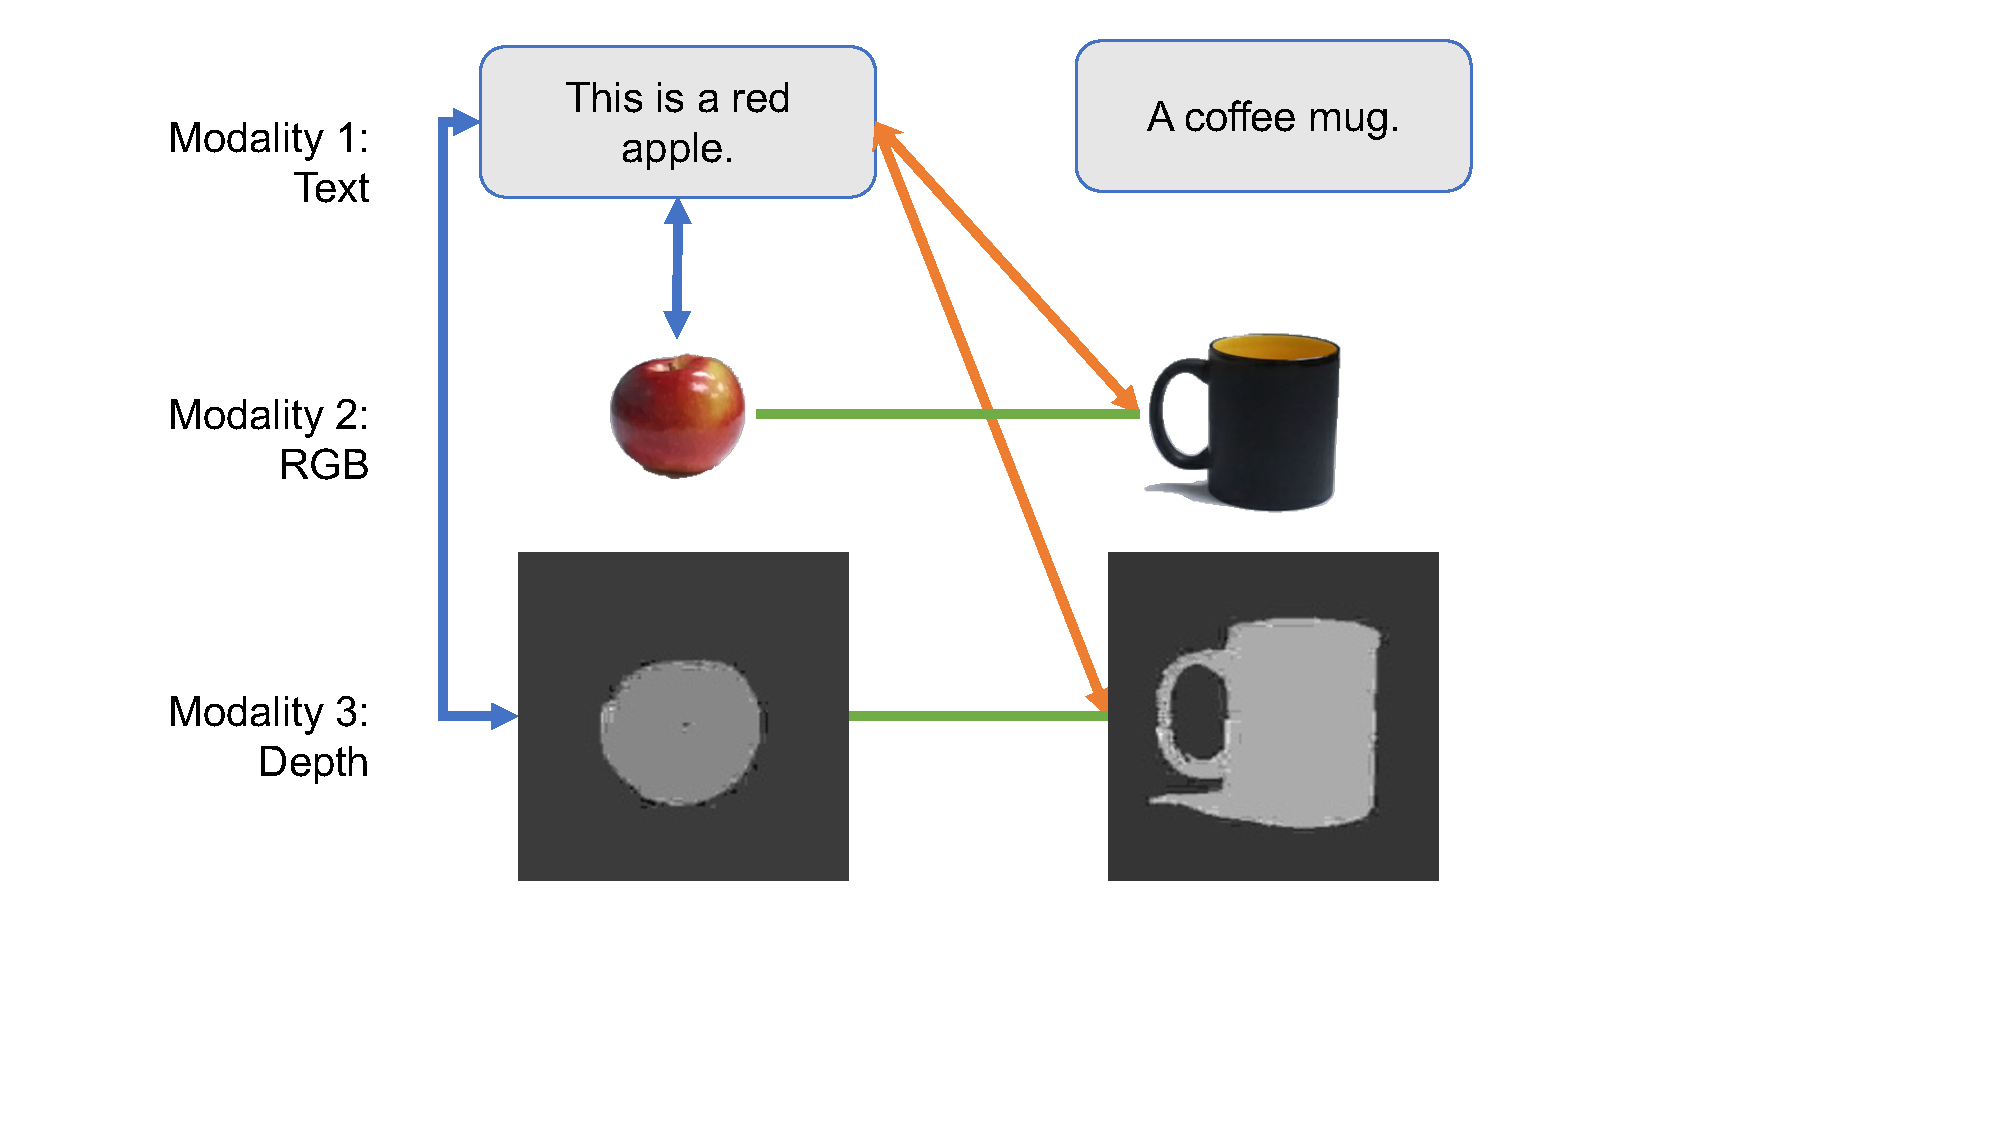
\includegraphics[width=\columnwidth]{Figures/simple-MMA.pdf}
\caption{A high-level prototype of the distances used in the simple MMA loss with 3 modalities. Orange arrows indicate maximizing the distance, blue arrows indicate minimizing the distance, and green lines show the margin. Depth images are brightened to be visible. \todo[inline]{We need to show speech as the 4th modality as well.}}
\label{fig:simple-mma-loss}
\end{figure}

This version of MMA loss function can be seen as a contrastive loss usually used in the domain of self-supervised learning~\cite{chen2020simple}. However, our proposed loss function has two advantages over the traditional contrastive loss expressed in equation~\ref{eq:contrastive-loss}. The first advantage is that our loss function do not loop over multiple positives and negatives in a large batch. Instead we sample only two objects (positive and negative) each of which have $M$ modalities which gives us $2M$ datapoints (or embeddings). Hence, our model can be trained using smaller batch sizes and reduces the number of negative samples we need. The second advantage is that this loss function can be used in a multimodal setting with an arbitrary number of modalities, and is not limited to a single data type (e.g. RGB images) which is the most common usage of contrastive loss~\cite{chen2020simple, NEURIPS2020_supervised_contrastive}.


Therefore, our proposed loss function would modify the equation~\ref{eq:contrastive-loss} to the loss function formulated in equation~\ref{eq:simple-MMA-contrastive}. Our formulation is a generalized version of the contrastive loss where $M$ is the number of modalities (e.g. RGB image, depth image, speech, text), but it can be the ``augmented views'' instead of different modalities.

% \begin{equation}\label{eq:simple-MMA-contrastive}
%     -\sum_{m=1}^{M-1} \log \frac{\exp (sim(f_a(x_a^+) , f_m(x_{m}^{+})/ \tau) )}{ \exp (sim(f_a(x_a^+) , f_m(x_{m}^{+}) / \tau)) + \exp (sim(f_a(x_a^+), f_m(x_{m}^{-}) / \tau))}
% \end{equation}

\begin{equation}\label{eq:simple-MMA-contrastive}
    -\sum_{m=1}^{M-1} \log \frac{\exp (sim(z_a^+ , z_{m}^{+})/ \tau) }{ \exp (sim(z_a^+ , z_{m}^{+}) / \tau) + \exp (sim(z_a^+, z_{m}^{-}) / \tau)}
\end{equation}
where $z = f(x)$.

% \todokdinline{I should run the traditional contrastive loss to see if my method works better to make this claim.}



% \subsubsection{All in loss with 12 terms}
% \subsubsection{subset of All in loss with 9 terms}

\subsection{EMMA}
\label{sub:emma}
In this version, we add the last term in equation~\ref{eq:objective} which maximizes the distance between positive and negative instances from the same modality. However, instead of looping over all modalities, we only do it for the anchor modality. The reason for that is because a margin between positive and negative points from other modalities (excluding anchor) is enforced. We formulate this method in equation~\ref{eq:objective-emma}.

This approaches closes the gap against supervised contrastive learning method when dropping speech, and increases the improvement even more when dropping text.

\begin{equation}
\label{eq:objective-emma}
\begin{split}
    \mathcal{L} = \sum_{m=1}^{M-1} \cos(z_{a}^{+} ,z_{m}^{-}) - \cos(z_{a}^{+}, z_{m}^{+}) - \cos(z_{a}^{+}, z_{a}^{-})
\end{split}
\end{equation}


\subsection{Network Architecture}
\label{sec:Model}

We use BERT~\cite{devlin-etal-2019-bert} embeddings from flair~\cite{akbik2019flair,akbik-etal-2019-pooled} to featurize the textual input, and wav2vec2~\cite{wav2vec2} to extract audio embeddings from speech both of which output a 3072-dimensional embedding vector.
To process images, we use ResNet152~\cite{He_resnet_2016} for both RGB and depth images which gives us a 2048-dimensional embedding vector.
We then use 3 fully connected layers with ReLU activation function~\cite{relu2010} to map these embeddings to a shared 1024-dimensional space where we can compute the distance between all embeddings.



%===================================================================


\section{Experiments}
\label{sec:Experiments}

We test our model against different baselines in different scenarios and settings using multiple metrics.

\subsection{Data}
\label{sec:Data}

We use a recent multimodal dataset called GoLD~\cite{GoLD_UMBC}. The original paper uses raw RGB and raw depth images in which other objects are present in the background. We use a masked version of the images where the background (including the white turntable) is deleted and one object is present in each image. We show that a masked version converges faster, however, they both converge to the same performance as shown in the supplementary material in figure~\ref{fig:mask-vs-raw}. Speech from GoLD is converted to 16 Hz in order to match wav2vec2 speech featurization model~\cite{wav2vec2}.





\subsection{Metrics}
\label{sec:metrics}
To evaluate our model we measure different performance metrics on a retrieval task where the model has to select an object among 5 objects given a language description. Only one of the objects corresponds to the description and the rest are from different object classes (e.g., one apple among a set including a fork, a mug, a lemon, and a bell pepper).

% \todokdinline{Try with different number of objects.}

To evaluate the performance, we compute the cosine distance between the given natural language description and 5 randomly selected images (1 of which corresponds to the description, with the others from different object classes). We handle depth images as a separate input modality (as opposed to appending depth to RGB, as others have done~\cite{triplet_loss_2021_CVPR}). We compute the distance between one textual language embedding and all candidate RGB embeddings, and we compute the distance between the same language embedding and all candidate depth embeddings corresponding to the RGB embeddings. We then take average of these two distance matrices. Instead of choosing an empirical threshold beyond which objects are considered to be `referred to,' we choose the closest image embedding (average distance of RGB and depth from language) as the prediction.

The best metric to capture the performance in such a scenario is mean reciprocal rank (MRR), in which the inverse of the rank of the correct object for a set of queries and then averaged. Accuracy, micro F1 score (sklearn), flattened binary f1 score (sklearn), and F1 score computation are all the same in this task, since for each prediction we either have a true positive and no false positives and no false negatives (no FP no FN), or we have no true positives and 1 false positive and 1 false negative. Subset MRR is equal or greater than those, because if the model does not rank the correct answer as 1, it still gets some score and is greater than 0 (in accuracy the score is ether 0 or 1).


\subsection{Setup}
\label{sec:setup}

Similar to~\citet{NEURIPS2020_supervised_contrastive}, we also use stochastic gradient descent (SGD) optimizer with momentum~\cite{ruder2016overviewSGD} with a flexible learning rate starting with 0.05.
The models are trained for 200 epochs with a batch size of 64 on a Quadro RTX 8000 GPU.
We use the same setup for all our experiments to have a fair comparison between different methods.



\subsection{4 Modalities}
We consider an experiment in which we incorporate RGB, depth, speech, and written language. The loss function requires no changes beyond increasing the number of loops in equation~\ref{eq:objective-simple-mma} (or increasing the value of $M$ by 1). Our goal is the non-trivial downstream prediction task: determining what objects are being referred to by arbitrary language from a small number of examples. In the case of three modalities, written language is used the anchor, and we compute the distance of RGB and depth modalities from it and then average them. However, when speech is incorporated as an additional sensory modality, we have three immediate possible choices. \textit{First}, we can treat speech in a similar way to RGB and depth: compute the distance of RGB, depth, and speech from text, and then take an average of three of them. \textit{Second}, we can compute the distance of RGB and depth from language and from speech which gives us 4 distance matrices, and then take average of these four. \textit{Third}, similar to the second method, we can compute the distance between language and speech as well and then take the average of 5 distance matrices. 

Of these, the first method is both more consistent with the goal of making a computationally tractable approach to arbitrary input modalities, and more consistent with existing work on using featurized speech directly as a sensory learning input; the simple MMA loss function in equation~\ref{eq:objective-simple-mma} is not designed to minimize the distance between speech and visual embeddings explicitly. This is supported by empirical results, in which the first method results in a better performance compared to the other two methods. 
% Third method (averaging 5 matrices) is the worst, then second one (averaging 4 matrices) is bad. First method has the best results.

\todokdinline{try the more complicated MMA that might be able to capture these relationships.}



\subsection{Baselines}
We compare our MMA model against different contrastive learning methods including the triplet loss~\cite{GoLD_UMBC, triplet_loss_2021_CVPR}, the traditional version of contrastive loss usually used in self-supervised settings~\cite{chen2020simple}, and supervised contrastive learning~\cite{NEURIPS2020_supervised_contrastive}. The triplet loss function consists of three data points including anchor, positive, and negative from two modalities. The anchor, positive, and negative can be chosen from different modalities in each batch.
The triplet loss method has two major disadvantages. First, it cannot be used for more than three modalities since there are only 3 data points in the loss function. Second, a batch size of greater than 1 cannot be easily implemented if the anchor, positive, and negative come from different modalities for each batch.
To address these issues, we sample more than one positive and one negative data points. Essentially, we sample one positive data point and one negative data point from each modality which results in 2(M-1) + 1 data points where 1 is the single anchor data point from anchor modality of the same object class as positive datapoints. We would have 2M datapoints if we use the negative data point from the anchor modality too. The anchor data point is always from the same modality and corresponds to the same object class sampled for positive data points.


\subsubsection{Contrastive Loss}
\label{sub:baseline-contrastive}

We compare our model against contrastive loss as formulated in equation~\ref{eq:contrastive-loss}. In order to implement this loss function, we use cosine similarity as suggested in the SimCLR paper~\cite{chen2020simple}. The other version (mentioned by~\citet{NEURIPS2020_supervised_contrastive}) uses an inner dot product that can lead to instabilities since the dot product is not bounded.
% \todokdinline{try contrastive loss with cross-entropy, dot product, and the supervised contrastive method itself (without triplets).}

% Original Formula
\begin{equation}\label{eq:contrastive-loss}
    -\sum_{i \in I} \log \frac{\exp (sim(z_i , z_{j(i)}) / \tau) }{\sum_{a \in A(i)} \exp (sim(z_i, z_a) / \tau)}
\end{equation}

% \begin{equation}\label{eq:contrastive-loss}
%     -\sum_{i \in I} \log \frac{\exp (sim(f(x_i) , z_{j(i)}) / \tau) }{\sum_{a \in A(i)} \exp (sim(f(x_i), f(x_a)) / \tau)}
% \end{equation}
where $i$ is anchor, $j(i)$ is the set of positives excluding anchor, $a$ is the set of all positives and negatives excluding anchor, and $z = f(x)$.

\subsubsection{Supervised Contrastive Learning}
\label{sub:baseline-supcon}

\citet{NEURIPS2020_supervised_contrastive} propose a supervised way of performing contrastive learning which is shown in equation~\ref{eq:supervised-contrastive}.

\begin{equation}\label{eq:supervised-contrastive}
    \sum_{i \in I} \frac{-1}{|P(i)|} \sum_{p \in P(i)} \log \frac{\exp (z_i \cdot z_p / \tau) }{\sum_{a \in A(i)} \exp (z_i \cdot z_a / \tau)}
\end{equation}

% \begin{equation}\label{eq:supervised-contrastive-my-notation}
%     \sum_{i \in I} \frac{-1}{|P(i)|} \sum_{p \in P(i)} \log \frac{\exp (f_i(x_i) \cdot f_p(x_p) / \tau) }{\sum_{a \in A(i)} \exp (f_i(x_i) \cdot f_a(x_a) / \tau)}
% \end{equation}


While this model is a strong baseline and the performance of our model is very close to this model, if the text modality is dropped, this method does not perform as good as our proposed model as shown in figure~\ref{fig:simple-MMA-mrr.srd}.


\begin{figure}[tbh]
\centering
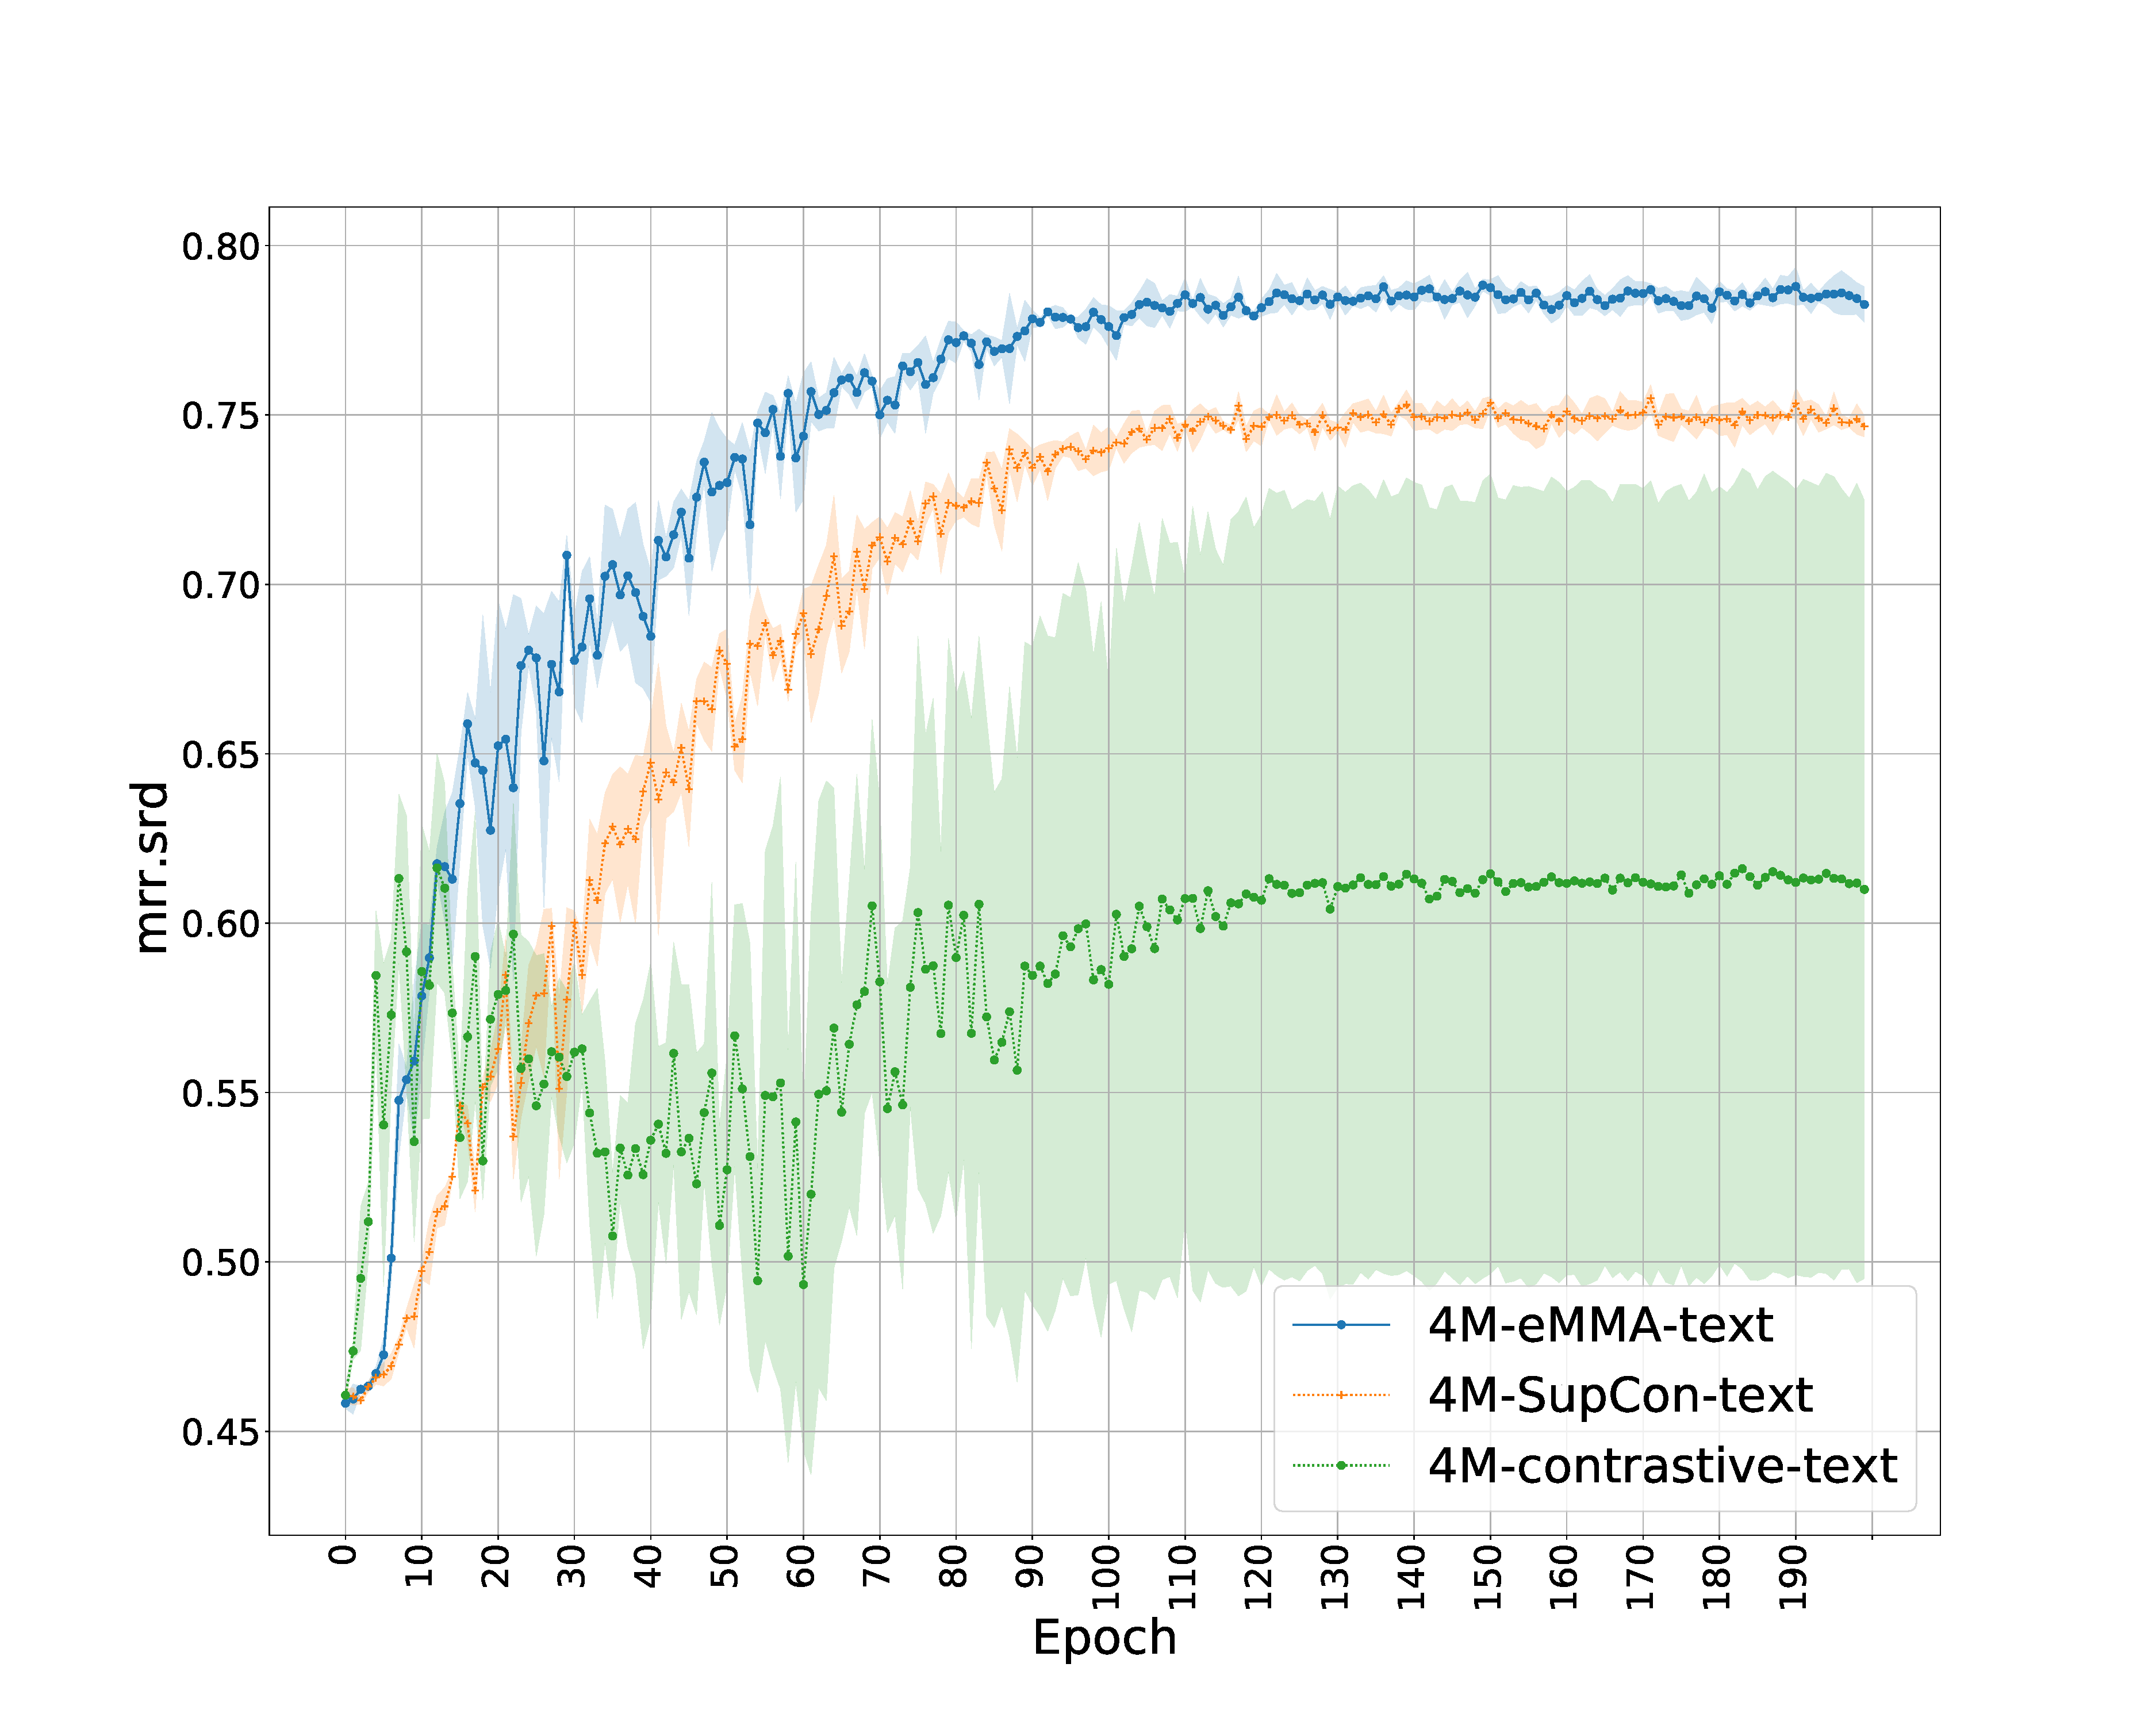
\includegraphics[width=.99\columnwidth]{Figures/average-seeds-epochs-mrr_ard.pdf}
\caption{Mean Reciprocal Rank (MRR) on the held-out test set when text modality is missing averaged over 3 runs with different random seeds. The higher is better. Green is Supervised Contrastive Learning~\cite{NEURIPS2020_supervised_contrastive} and pink represents our proposed simple MMA loss function without semantic negative sampling w/ SGD w/ adjusting learning rate.
% \todokdinline{Add legend to the graph.}
}

\label{fig:simple-MMA-mrr.srd}
\end{figure}




\subsection{Quantitative Results}
\label{sec:Quantitative}

We evaluate our proposed simple MMA loss function~\ref{sub:simple-mma} against the triplet loss method~\cite{triplet_loss_2021_CVPR}. Our model significantly outperforms the triplet method across all epochs while it converges faster as shown in figure~\ref{fig:simple-MMA-mrr}.
Table~\ref{table:quantitative} summarizes the performance of all models.

\begin{table*}[tbh]
\centering
\begin{tabular}{|c|c|c|c|c|c|}
\toprule
\textbf{Method} & \textbf{Modalities} & \textbf{Accuracy} & \textbf{MRR.srd} & \textbf{MRR.trd} & \textbf{MRR.tsrd} \\ %\hline
\midrule
Simple MMA (Text) w/o neg  SGD & 3 & 0.8168$\pm$? & 0.8962$\pm$? & ? & ? \\
eMMA (Text) w/o neg SGD & 3 & 0.8168$\pm$? & 0.8962$\pm$? & ? & ? \\
Contrastive Cosine (Text) w/ neg & 3 & 0.7894$\pm$? & 0.8788$\pm$?  & ? & ?\\
Supervised Contrastive (Text)& 3 & 0.8332$\pm$? & 0.9057$\pm$? & ? & ?\\
Simple MMA (Text) w/o neg  SGD & 4 & ?$\pm$? & ?$\pm$? & ? & ? \\
Supervised Contrastive (Text)& 4 & ?$\pm$? & ?$\pm$? & ? & ? \\
Simple MMA (Speech) w/o neg & 3 & 0.7949$\pm$? & 0.8778$\pm$? & ? & ?  \\
Triplet (Speech) w/o neg & 3 & 0.7497$\pm$? & 0.8522$\pm$? & ? & -  \\
% Full MMA (Text) w/ neg & 3 & ?$\pm$? & ?$\pm$? \\
% Simple MMA (Text) w/ neg Adam & 3  & 0.7949$\pm$? & 0.8778$\pm$? \\
% Simple MMA (Text) w/ neg SGD & 3 & 0.7905$\pm$? & 0.8821$\pm$? \\
% Triplet (Text) w/ neg & 3 & 0.7497$\pm$? & 0.8522$\pm$? \\
% Full MMA (Speech) w/ neg & 3 & ?$\pm$? & ?$\pm$? \\
% Simple MMA (Speech) w/ neg & 3 & 0.7949$\pm$? & 0.8778$\pm$? \\
% Contrastive (Speech) w/ neg & 3 & ?$\pm$? & ?$\pm$? \\
% Triplet (Speech) w/ neg & 3 & 0.7497$\pm$? & 0.8522$\pm$? \\
\bottomrule
\end{tabular}
\caption{\label{table:quantitative}Average and standard deviation of accuracy and MRR over 3 runs with 3 different random seeds on a held-out test set. Both metrics are from 0 to 1, and the higher is better.
% \todokdinline{maybe adding results on cropped and raw dataset as well. Also results using object class instead of negative sampling}
}
\end{table*}


\begin{figure}[tbh]
\centering
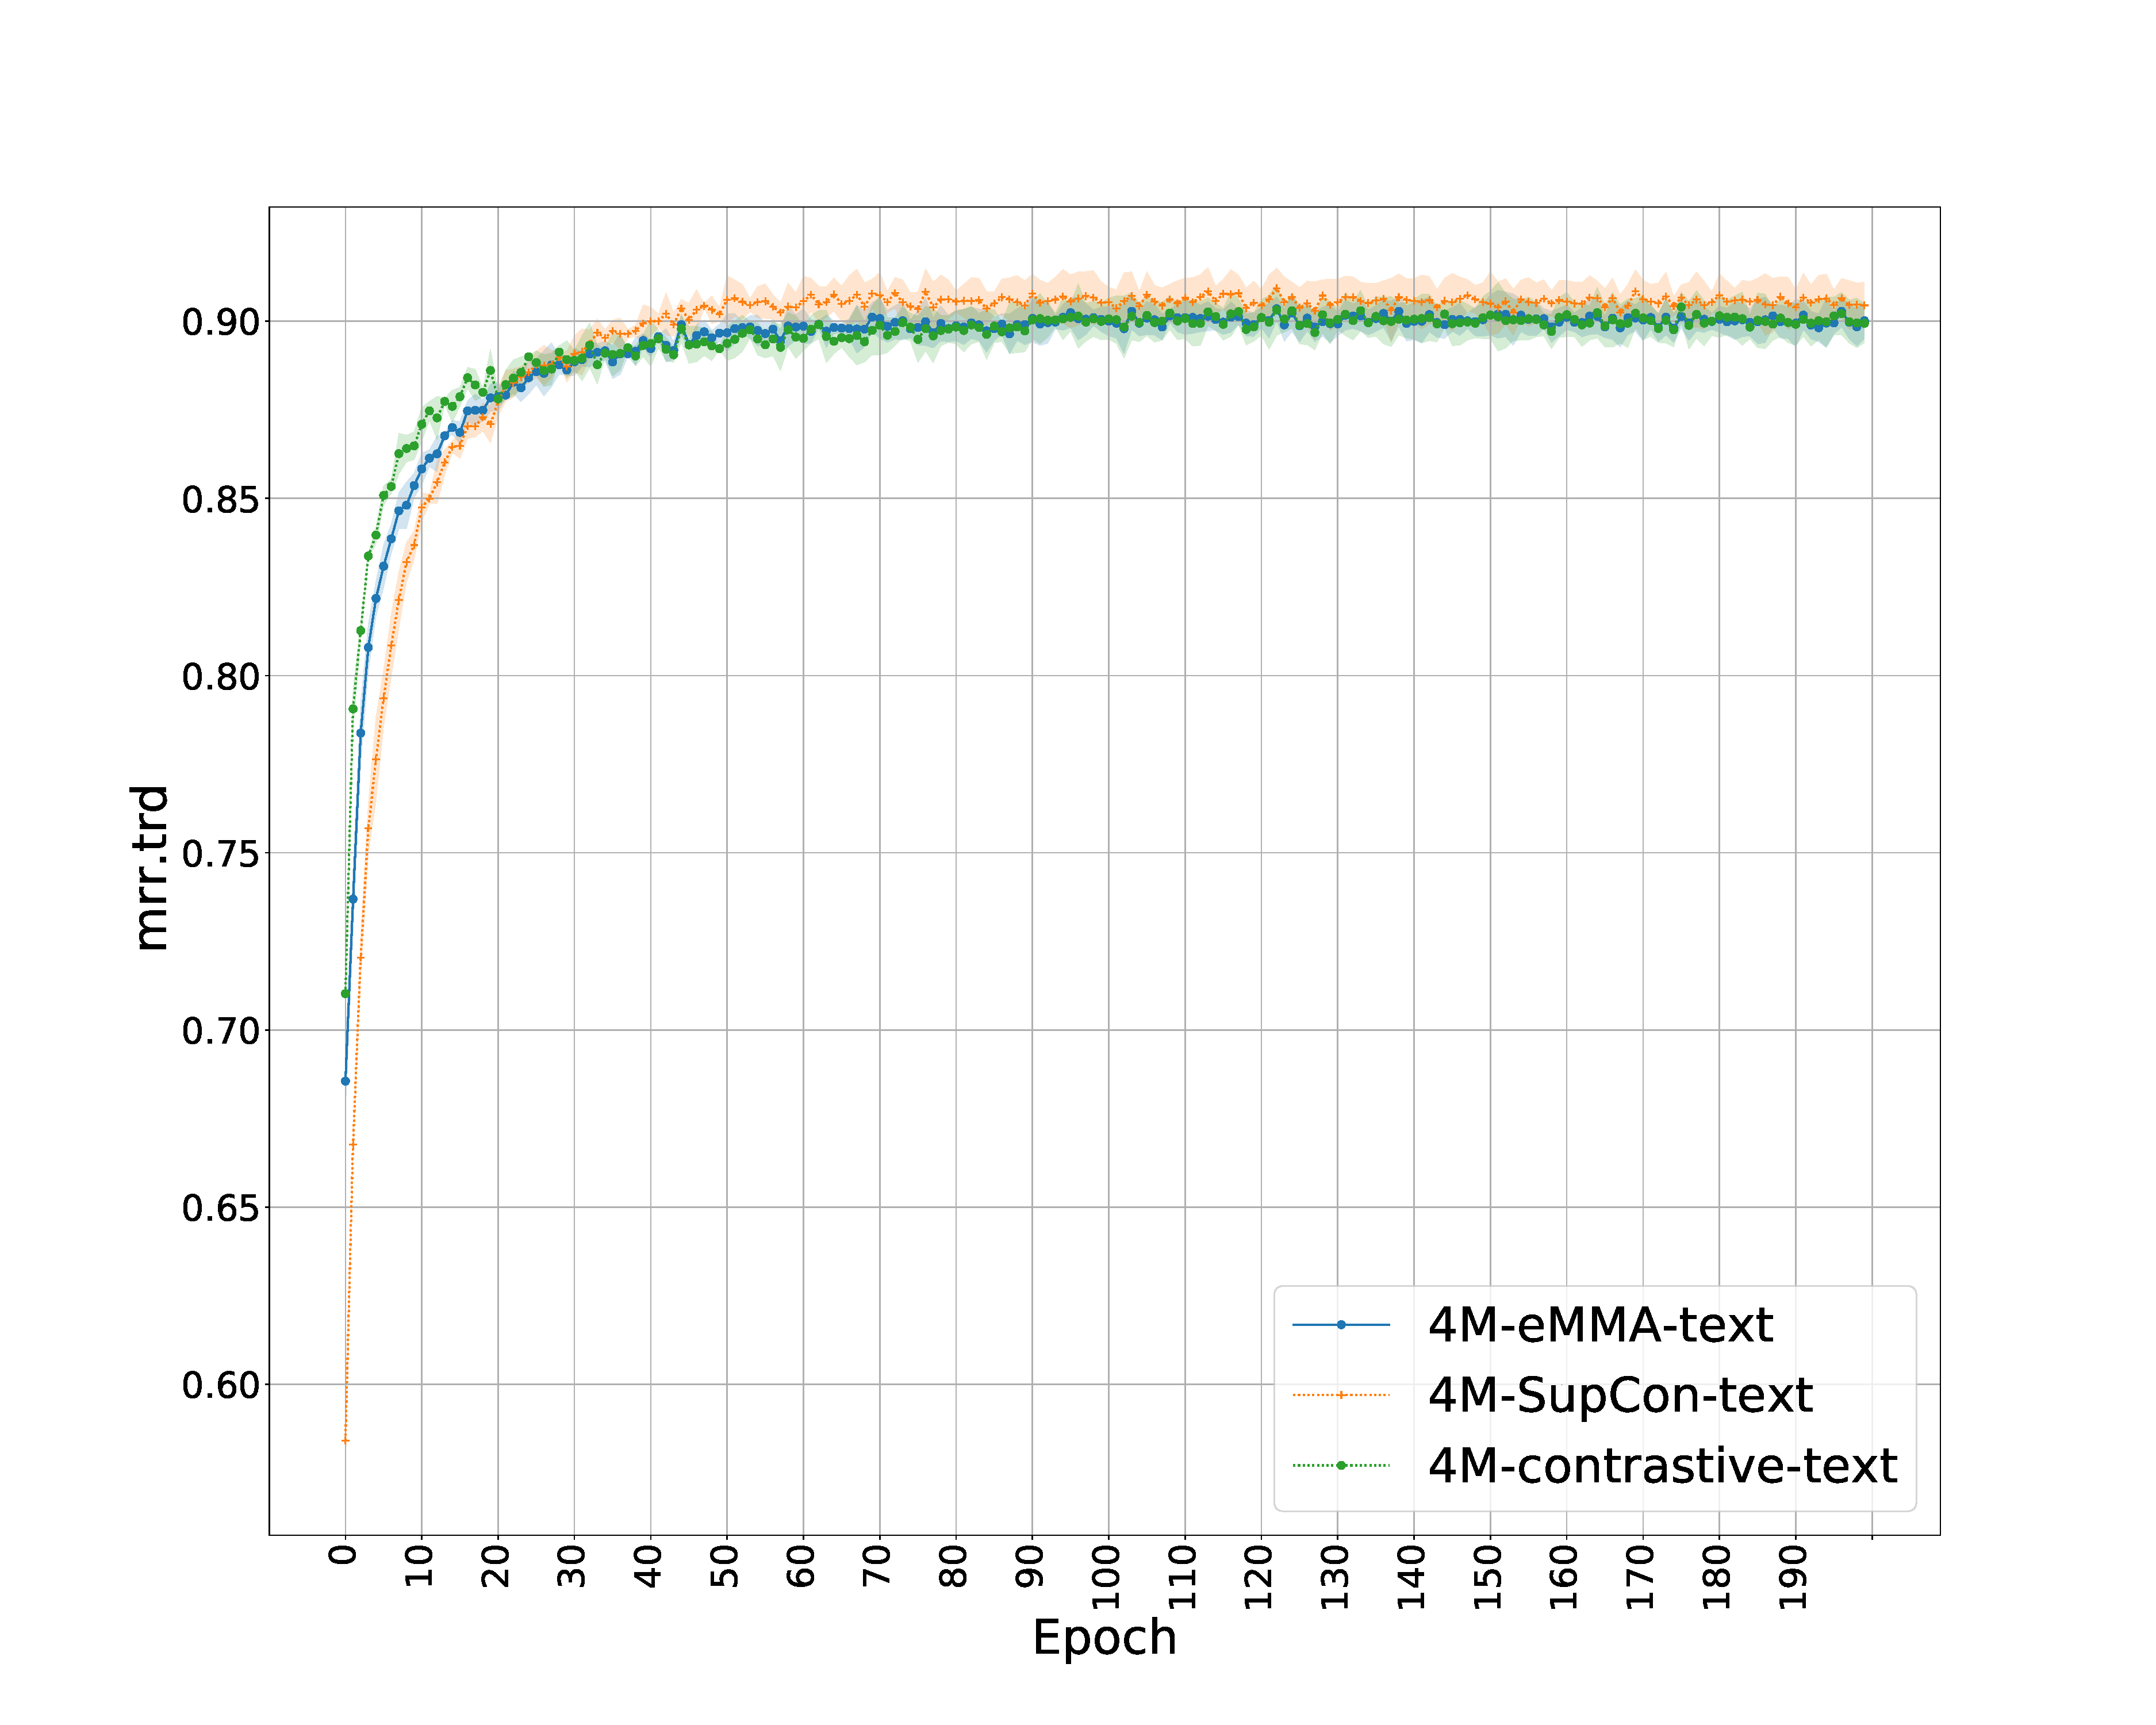
\includegraphics[width=.99\columnwidth]{Figures/average-seeds-epochs-mrr_lrd.pdf}
\caption{Mean Reciprocal Rank (MRR) on the held-out test set when speech modality is dropped averaged over 3 runs with different random seeds for a downstream task of object retrieval. The higher is better. Orange represents Supervised Contrastive Learning~\cite{NEURIPS2020_supervised_contrastive}, \Complete{} represents the triplet loss function~\cite{triplet_loss_2021_CVPR}.
\todokdinline{remove simple MMA and probably add triplet loss. Any ideas?}
}
% \todocmi{Maybe MRR is wrong and we should be looking at top-ranked result?}
\label{fig:simple-MMA-mrr}
\end{figure}


\subsection{Qualitative Results}
\label{sec:Qualitative}

\begin{enumerate}
    \item DONE Perform t-sne visualization of embeddings.
    \item TODO Dropout modalities MRR
\end{enumerate}





\subsection{Failed Experiments}
We tried a lot of different approaches and they did not work better than our model or the baselines, but we list them here to save time for readers who want to try them.

\subsubsection{Two Anchors}
Since speech is similar to text in its usage when it comes to the downstream task of object retrieval (given a single language command, find the correct object among multiple objects), we decided to have text and speech as two anchors instead of having one anchor only. When there is one anchor, the distance between positive pairs text and speech is minimized and the distance between negative pairs are minimized. However, this is not related to the downstream task since we never want to find the correct speech for a given text or vice versa. The second term added to the last function is exactly similar to the loss function when speech is the anchor, and the first term is the same as when language is the anchor. Therefore, the performance is somewhere in the middle of those two approaches but more towards the speech when the metrics are computed based and speech matrices.




%===================================================================





\section{Conclusion}
\label{sec:conclusion}


%===================================================================


% ***************** The END of the paper *****************

% %% The acknowledgments section is defined using the "acks" environment
% %% (and NOT an unnumbered section). This ensures the proper
% %% identification of the section in the article metadata, and the
% %% consistent spelling of the heading.
\begin{acks}
To Robert, for the bagels and explaining CMYK and color spaces.
\end{acks}
% \section*{Acknowledgments}



\clearpage
\clearpage
% %%
% %% The next two lines define the bibliography style to be used, and
% %% the bibliography file.
\bibliographystyle{ACM-Reference-Format}
\bibliography{ref}

% %%
% %% If your work has an appendix, this is the place to put it.
\appendix
\label{sec:appendix}


\section{Qualitative Analysis}
\section{Model}


\section{Data}

\begin{figure*}[tbh]
\centering
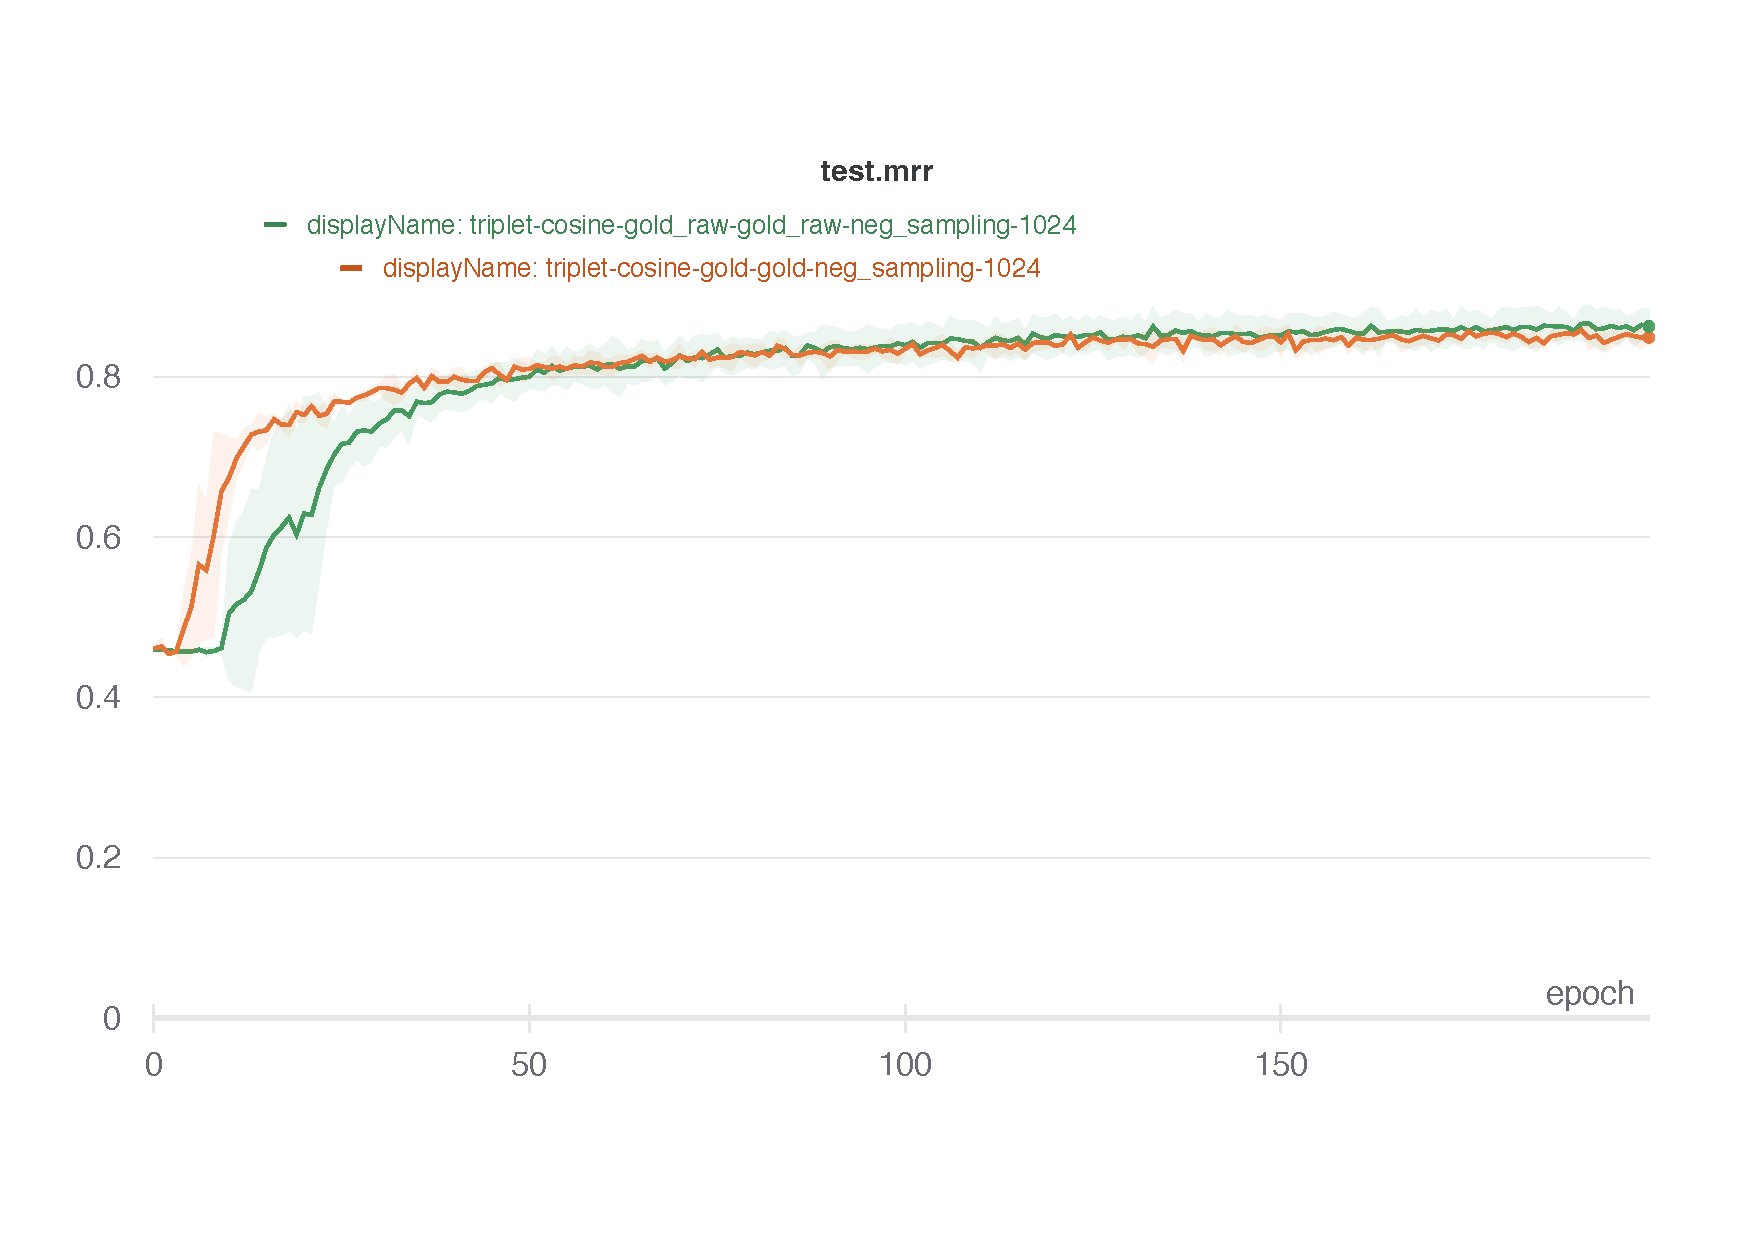
\includegraphics[width=2.0\columnwidth]{Figures/raw-mask-test-mrr.pdf}
\caption{Mean Reciprocal Rank (MRR) on different versions of GoLD dataset~\cite{GoLD_UMBC}. The raw version is depicted in green and masked version is depicted in orange averaged over 3 different random seeds. Higher is better.}
\label{fig:mask-vs-raw}
\end{figure*}

\section{Experiments}

\section{Results}

\begin{figure*}[tbh]
\centering
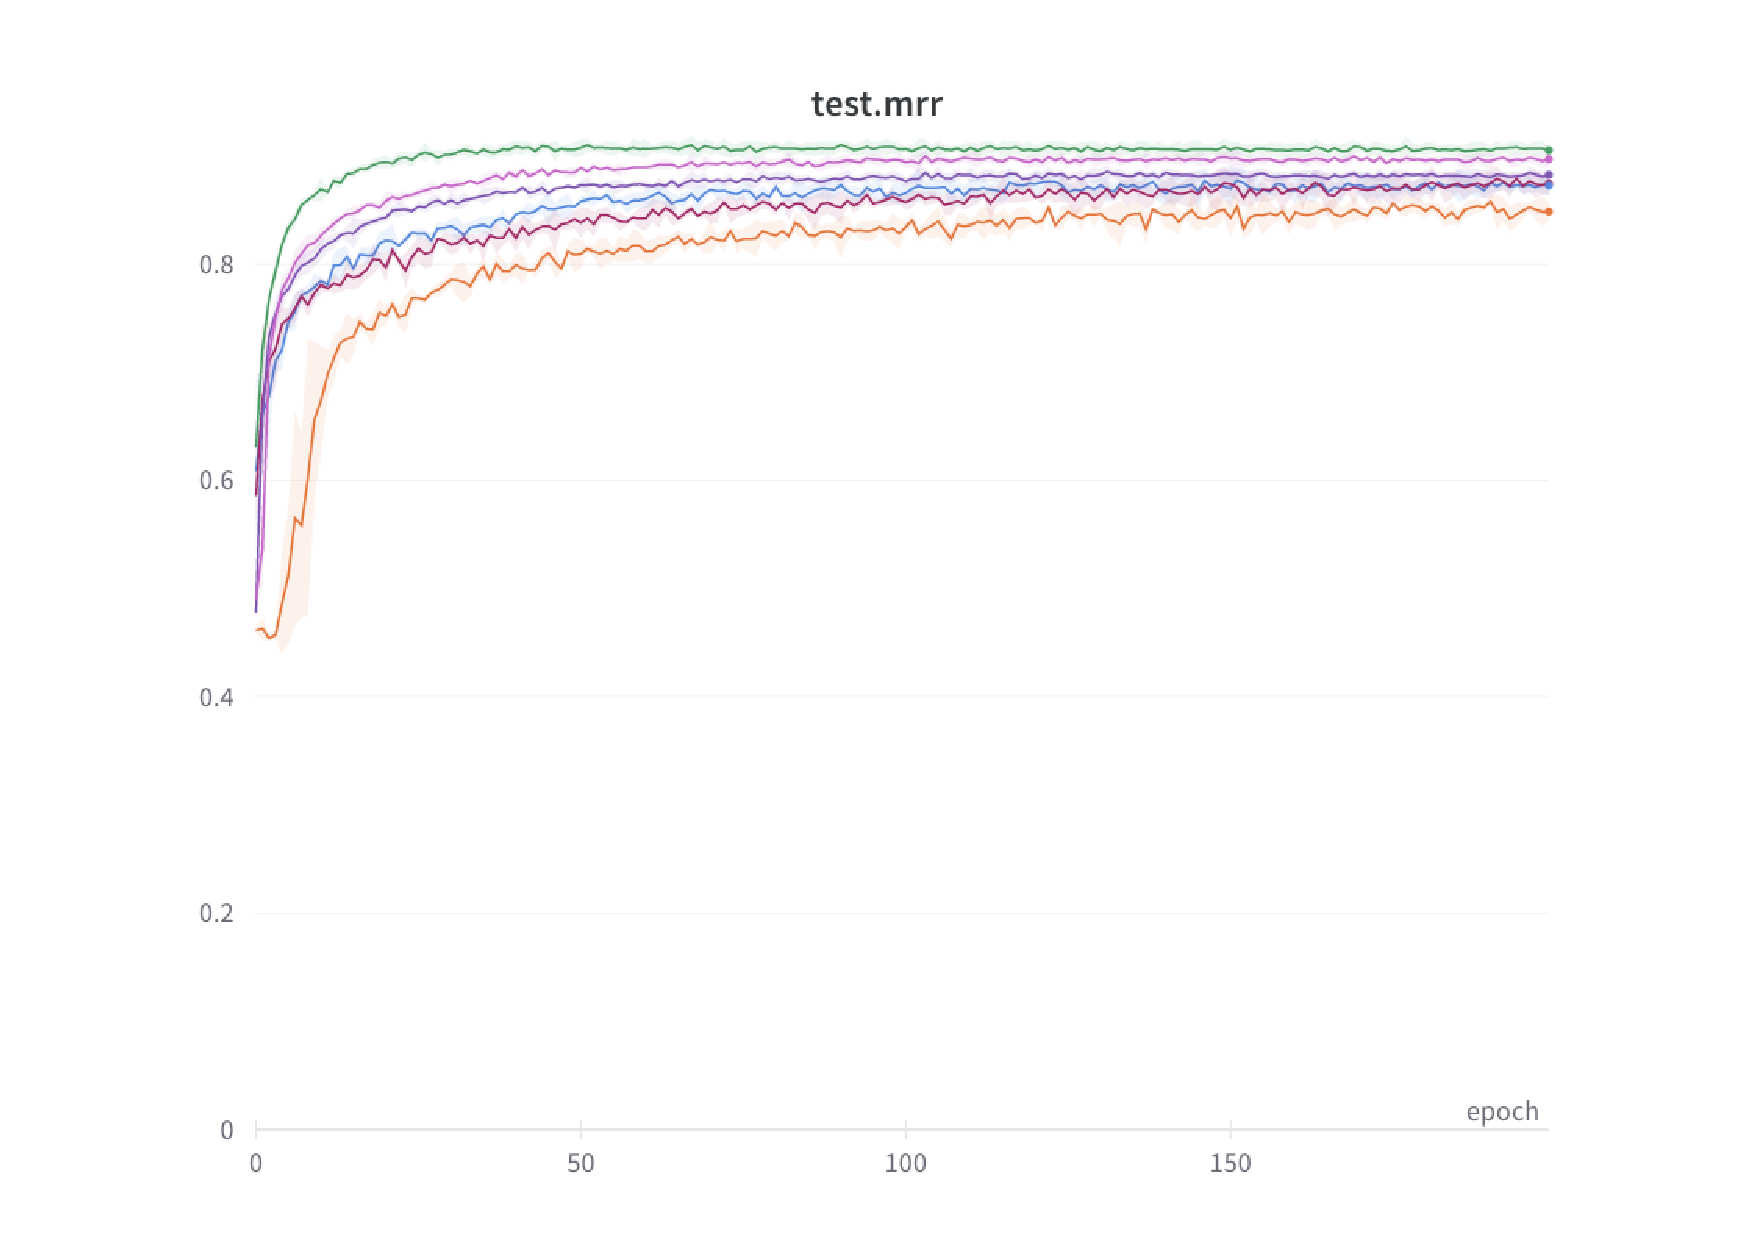
\includegraphics[width=2.1\columnwidth]{Figures/test.mrr.pdf}
\caption{Mean Reciprocal Rank (MRR) of our proposed method against triplet loss method averaged over 3 different random seeds for a downstream task of object detection. The higher is better. Green is Supervised Contrastive Learning~\cite{NEURIPS2020_supervised_contrastive}, Pink represents our proposed simple MMA loss function without semantic negative sampling w/ SGD w/ adjusting learning rate, Purple is out method with semantic negative sampling, Blue is our method w/ semantic negative sampling w/ Adam and w/o adjusting learning rate, Red is vanilla contrastive loss with cosine, and orange represent the triplet loss. function~\cite{triplet_loss_2021_CVPR}.
}

\label{fig:simple-MMA-mrr}
\end{figure*}

\section{Setup}

% \section{Lit Search}
\subsection{Multimodal Machine Learning: A Survey and Taxonomy}

\begin{itemize}
\item \href{https://ieeexplore.ieee.org/document/8269806}{url}
\end{itemize}

\citet{baltrusaitisMultimodalMachineLearning2019} proposes a new taxonomy of multimodal machine learning by introducing five technical challenges in addition to typical early and late fusion categorization. This taxonomy includes the following categories.
\begin{enumerate}
\item \textit{Representation}: represent and summarize multimodal data in a way that exploits the complementarity and redundancy of multiple modalities.
\begin{enumerate}
\item joint: combine the unimodal signals into the same representation space.
\item coordinated: process unimodal signals separately, but enforce certain similarity or structure constraints on them to bring them to a coordinated space.
\end{enumerate}
\item \textit{Translation}: map data from one modality to another.
\begin{enumerate}
\item example-based
\item generative
\end{enumerate}
\item \textit{Alignment}: identify the direct relations between (sub)elements from two or more different modalities.
\begin{enumerate}
\item explicit
\item implicit
\end{enumerate}
\item \textit{Fusion}: join information from two or more modalities to perform a prediction.
\begin{enumerate}
\item model-agnostic
\item model-based
\end{enumerate}
\item \textit{Co-learning}: transfer knowledge between modalities, their representation, and their predictive models
\begin{enumerate}
\item parallel data
\item non-parallel data
\item hybrid data
\end{enumerate}
\end{enumerate}

The authors mention that while joint representations have been used in situations to construct representations of more than two modalities, coordinated spaces have, so far, been mostly limited to two. This means that our research is novel and we can extend similarity measures to more than two modalities.

\subsection{Self-Supervised MultiModal Versatile Networks}

\begin{itemize}
\item \href{https://proceedings.neurips.cc/paper/2020/file/0060ef47b12160b9198302ebdb144dcf-Paper.pdf?utm\_campaign=NLP\%20News\&utm\_medium=email\&utm\_source=Revue\%20newsletter}{url}
\end{itemize}


This work uses self-supervised contrastive learning to learn and combine representations from three modalities of visual, audio, and language. They learn a \textit{multimodal versatile network} that has the following four properties:
\begin{enumerate}
\item Ability to take any of the modalities as input
\item Respecting the specificity of modalities: audio and visual modalities are fine-grained while language modality is coarse-grained.
\item Comparability of different modalities using \textbf{dot product} even if not seen together during training 
\item Efficiently applicable to visual data either in the form of dynamic videos or static images
\end{enumerate}


The authors consider the following three different configurations of the modality spaces which they call \textit{modality embedding graphs}.
\begin{enumerate}
\item Shared: all modalities map to the same space. This respects property 3 but violates property 2.
\item Disjoint: visual-audio and visual-text spaces. This respects property 2 but violates property 3.
\item Fine and coarse: audio and visual domains are map to the same space since they are fine-grained. These embeddings are then mapped to a lower dimensional space where text is also mapped. This respects both properties 2 and 3.
\end{enumerate}

The loss function they define consists of two terms. The first term is to train the fine-grained space of visual and audio embeddings by minimizing the distance between the similar pair (positives) from the same location of a video, and maximizing the distance between negative pairs (negatives) sampled from different videos. The second term is to train the coarse-grained space which consists of visual and text embeddings. Note that they don't consider audio embeddings in this space since they don't want to learn automatic speech recognition (ASR). Text and visual domains are not aligned as well as audio and visual domains (e.g. sound of playing piano versus the text that only says playing piano for a video of playing piano). To cure this, they consider a set of positive pairs instead of a single pair.
If a modality is missed, the corresponding term is dropped from the loss function.

\subsection{Separating Self-Expression and Visual Content in Hashtag Supervision}

\begin{itemize}
\item \href{https://openaccess.thecvf.com/content\_cvpr\_2018/papers/Veit\_Separating\_Self-Expression\_and\_CVPR\_2018\_paper.pdf}{url}
\end{itemize}

The authors train a joint model of images, hashtags, and users to perform image retrieval. This is similar to our task where given a description, we want to find the image in the scene that best matches the description. The idea is to form a three-way tensor product model. They use a ranking loss to train the model where the score of an observed triplet is higher than an unobserved triplet. They sample six negative triplets per positive sample triplet, and use each of them as a negative in the loss.
The downstream retrieval task is then simply done by taking the arg max of the tensor product for a given user.



\subsection{Semi-Heterogeneous Three-Way Joint Embedding Network for Sketch-Based Image Retrieval}

\begin{itemize}
\item \href{https://ieeexplore.ieee.org/document/8809264}{url}
\end{itemize}

\subsection{Deep Multimodal Learning for Affective Analysis and Retrieval}

\begin{itemize}
\item \href{https://ieeexplore.ieee.org/abstract/document/7277066?casa\_token=aBp6BxcszHwAAAAA:3NoMiFrZbn7tXfavF1rgkCiGWbFI2arxn8Xb6iDF79q4zBZHWi7PWWhf6xW-xJwYdFALbmRENo4}{url}
\end{itemize}

\subsection{An Efficient Framework for Zero-Shot Sketch-Based Image Retrieval}

\begin{itemize}
\item \href{https://arxiv.org/pdf/2102.04016.pdf}{url}
\end{itemize}
This paper uses two modalities only; image and sketch. However, it uses a \textit{quadruplet} to compute the loss which can be useful in our research. A quadruplet is composed of a sketch picture as an anchor, a negative example from sketch domain, a negative example from picture domain, and a positive example from picture domain.

\subsection{SMIL: Multimodal Learning with Severely Missing Modality}

\begin{itemize}
\item \href{https://www.aaai.org/AAAI21Papers/AAAI-437.MaM.pdf}{url}
\end{itemize}
Uses Bayesian meta-learning framework to perform multimodal learning with partially missing modalities in training/test data.
One of their experiments is multi-label classification of movie genres with bimodal data including poster of movies and description of the movie from IMDB.

\subsection{Multimodal Language Analysis in the Wild: CMU-MOSEI Dataset and Interpretable Dynamic Fusion Graph}

\begin{itemize}
\item \href{https://aclanthology.org/P18-1208.pdf}{url}
\end{itemize}

\subsection{Multimodal Learning with Incomplete Modalities by Knowledge Distillation}

\begin{itemize}
\item \href{https://dl.acm.org/doi/pdf/10.1145/3394486.3403234}{url}
\end{itemize}
They first train models on each modality independently
\subsection{SWAFN: Sentimental Words Aware Fusion Network for Multimodal Sentiment Analysis}

\begin{itemize}
\item \href{https://aclanthology.org/2020.coling-main.93.pdf}{url}
\end{itemize}

\subsection{Multimodal Learning for Human Action Recognition Via Bimodal/Multimodal Hybrid Centroid Canonical Correlation Analysis}

\begin{itemize}
\item \href{https://ieeexplore.ieee.org/document/8489981}{url}
\end{itemize}

\subsection{Deception Detection Using a Multimodal Approach}

\begin{itemize}
\item \href{https://dl.acm.org/doi/pdf/10.1145/2663204.2663229?casa\_token=KneK7B7xvLwAAAAA:Ajz0N96ygq8ktwkz0IVUqTt8NozCg2wR6n\_x2xntdHqZBh6VXW\_8VbO4GeY4VvMsDJlMwzkhVXQSJA}{url}
\end{itemize}
They use \textit{language}, \textit{physiological response}, and \textit{thermal sensing} to detect deceit.

\subsection{M3ER: Multiplicative Multimodal Emotion Recognition using Facial, Textual, and Speech Cues}

\begin{itemize}
\item \href{https://ojs.aaai.org/index.php/AAAI/article/view/5492}{url}
\end{itemize}

\subsection{Found in Translation: Learning Robust Joint Representations by Cyclic Translations between Modalities}

\begin{itemize}
\item \href{https://ojs.aaai.org/index.php/AAAI/article/view/4666}{url}
\end{itemize}
\subsection{Select-Additive Learning: Improving Generalization In Multimodal Sentiment Analysis}

\begin{itemize}
\item \href{https://ieeexplore.ieee.org/stamp/stamp.jsp?tp=\&arnumber=8019301}{url}
\end{itemize}

\subsection{Attention-Based Multimodal Fusion for Video Description}

\begin{itemize}
\item \href{https://openaccess.thecvf.com/content\_ICCV\_2017/papers/Hori\_Attention-Based\_Multimodal\_Fusion\_ICCV\_2017\_paper.pdf}{url}
\end{itemize}
\subsection{\st{3W-AlignNet: a Feature Alignment Framework for Person Search with Three-Way Decision Theory}}

\begin{itemize}
\item \href{https://link.springer.com/article/10.1007/s12559-021-09898-7}{url}
\end{itemize}

This is not very related since they use three-way decision theory to select bounding boxes as positive, negative, and boundary.
Three-way here refers to something else and not modalities.

\subsection{\st{Unsupervised Domain Adaptation for Face Recognition in Unlabeled Videos}}
\begin{itemize}
\item \href{https://openaccess.thecvf.com/content\_ICCV\_2017/papers/Sohn\_Unsupervised\_Domain\_Adaptation\_ICCV\_2017\_paper.pdf}{url}
\end{itemize}
Might be relevant but not super relevant.


\subsection{Heterogeneous Sensor Data Fusion By Deep Multimodal Encoding}
\begin{itemize}
\item \href{https://ieeexplore.ieee.org/stamp/stamp.jsp?tp=&arnumber=7874158}{url}
\end{itemize}
This one takes two modalities as input and outputs predictions in a third modality.

\subsection{Multimodal Contrastive Training for Visual Representation Learning}
\href{https://arxiv.org/pdf/2104.12836.pdf}{paper pdf}


\subsection{CrossCLR: Cross-modal Contrastive Learning For Multi-modal Video Representations}
\href{https://openaccess.thecvf.com/content/ICCV2021/papers/Zolfaghari_CrossCLR_Cross-Modal_Contrastive_Learning_for_Multi-Modal_Video_Representations_ICCV_2021_paper.pdf}{paper pdf}

%===================================================================





\end{document}

